\documentclass{article}

\usepackage{amsmath,amssymb,amsthm}
\usepackage{tikz}
\usepackage{graphicx}
\usetikzlibrary{arrows,graphs}

\setlength{\oddsidemargin}{0.25 in}
\setlength{\evensidemargin}{-0.25 in}
\setlength{\topmargin}{-0.6 in}
\setlength{\textwidth}{6.5 in}
\setlength{\textheight}{8.5 in}
\setlength{\headsep}{0.75 in}
\setlength{\parindent}{0 in}
\setlength{\parskip}{0.1 in}

\newtheorem{theorem}{Theorem}
\newtheorem{corollary}{Corollary}
\newtheorem{proposition}{Proposition}
\newtheorem*{remark}{Remark}
\theoremstyle{definition}
\newtheorem{example}{Example}
\newtheorem{definition}{Definition}

\newcommand{\lecture}[4]{
   \pagestyle{myheadings}
   \thispagestyle{plain}
   \newpage
%   \setcounter{lecnum}{#1}
   \setcounter{page}{1}
   \noindent
   \begin{center}
   \framebox{
      \vbox{\vspace{2mm}
    \hbox to 6.58in { {\bf CSC~565: Graph Theory
                        \hfill North Carolina State University} }
    \hbox to 6.58in { {\bf Fall 2019
                        \hfill Computer Science} }
       \vspace{4mm}
       \hbox to 6.28in { {\Large \hfill Lecture #1: #2  \hfill} }
       \vspace{2mm}
       \hbox to 6.28in { {\it Lecturer: {\it Don Sheehy {\tt <drsheehy@ncsu.edu>}} \hfill Scribe: #4} }
      \vspace{2mm}}
   }
   \end{center}
   \markboth{Lecture #1: #2}{Lecture #1: #2}
   \vspace*{4mm}
}


\begin{document}

  \title{Lecture 13}
  \author{Scribed by: Erik Rosenstrom, Maharshi Parekh, Sichao Yu, Yunxuan Shi }
  \date{October 9, 2019}
  \maketitle


  \begin{theorem}
    [The Fary] If G is a planar, then there exists a linear embedding of G.
  \end{theorem}
  \begin{proof}
    It suffices to consider maximal planar graphs.
  

  \begin{figure}[htp]
    \centering % 图片居中
    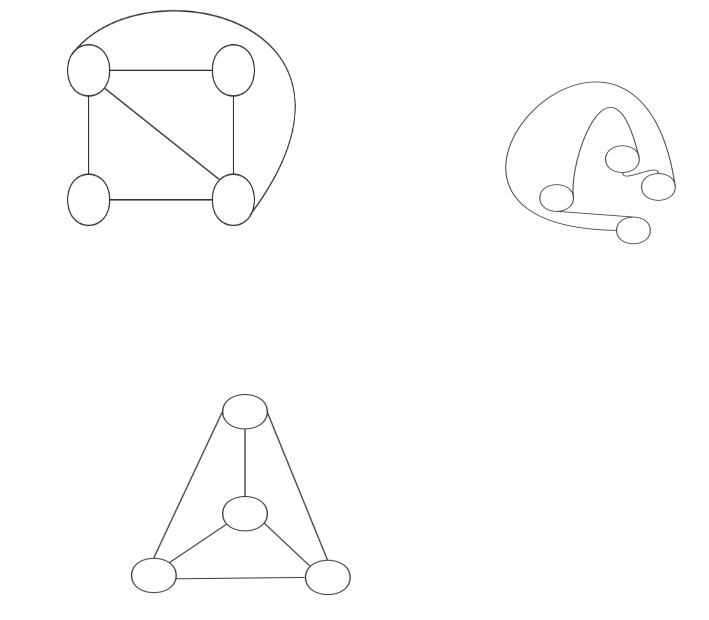
\includegraphics[width = 8.3cm]{week8/figure/fary.jpg}
    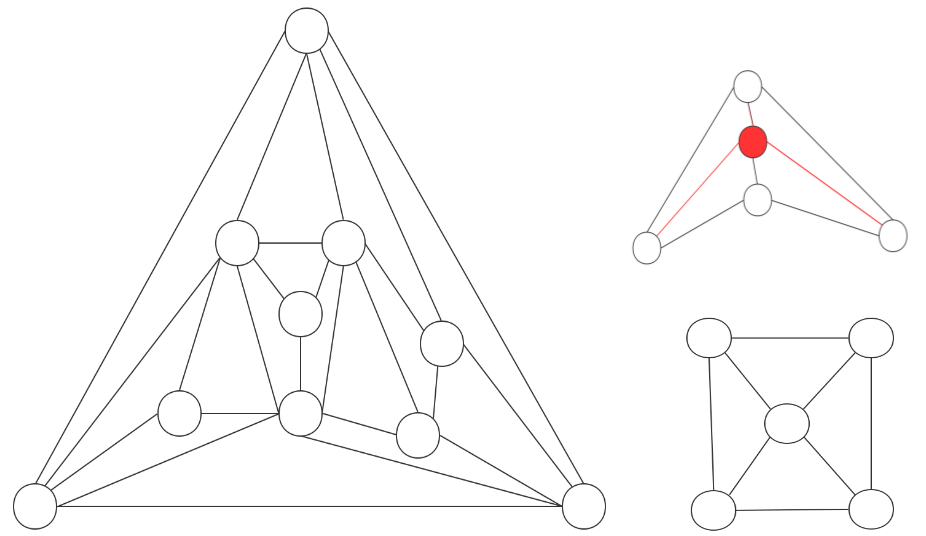
\includegraphics[width = 8.3cm]{week8/figure/fary2.jpg}
  \end{figure}
  
  
  \begin{defination}
    [star-shaped polygons]. Polygon P is a star-shaped if there exists \[x\in  int(P)\] Such that \[ \bar{xy}\in P for \ all \ y \in P\]
    Claim: All 5-gons are star-shaped
   \end{defination}   
    
  \begin{figure}[htp]
    \centering % 图片居中
    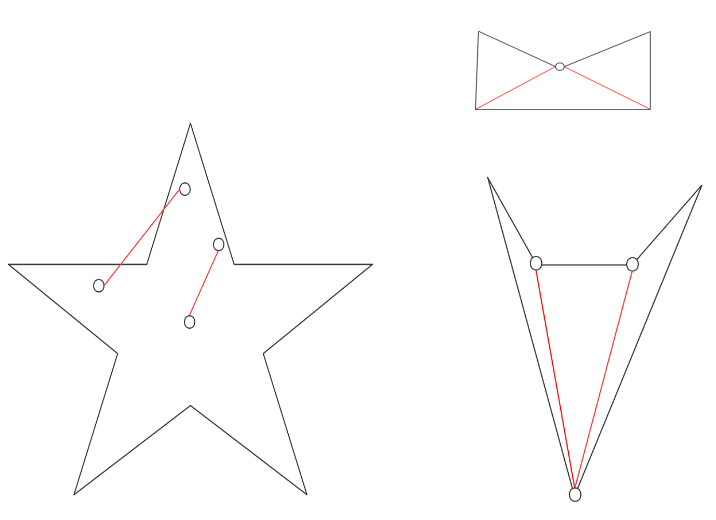
\includegraphics[width = 8.3cm]{week8/figure/5-gons1.jpg}
    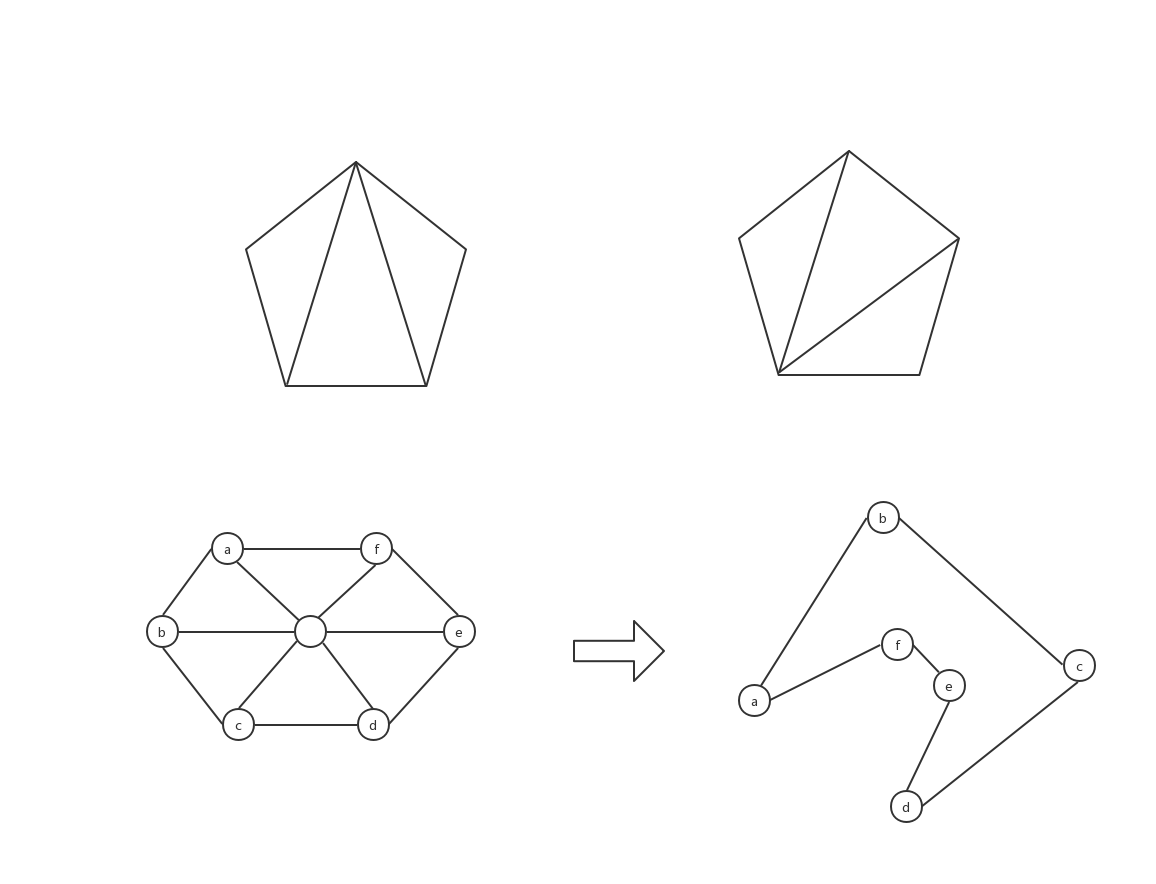
\includegraphics[width = 8.3cm]{week8/figure/5-gons2.jpg}
  \end{figure}
    
    Since every planar graph has at least one vertex with \(deg(v)\leq 5 \).
    Let \(v\) be a vertex with \(deg(v)\leq 5 \). \(G'\) is \(G\setminus v\) plus 2 edges to make it maximal. 
    \begin{figure}[!h]
      \centering
      {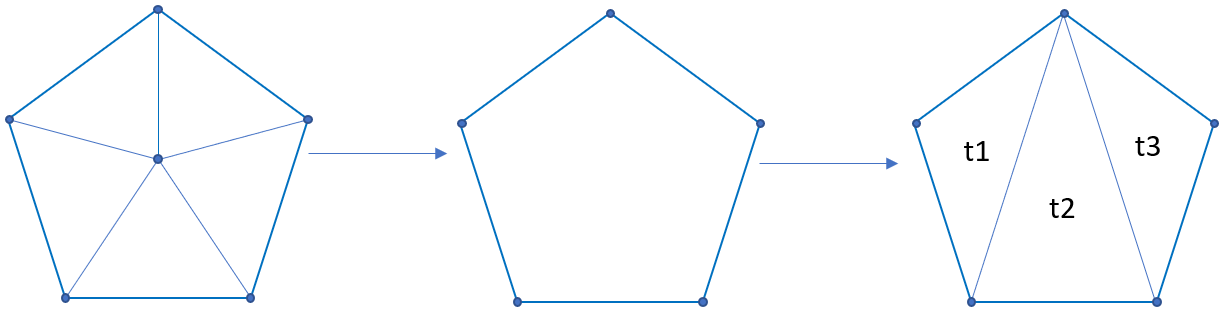
\includegraphics[width=0.7\textwidth]{figure/pentagon.png}}
      \caption{Remove a vertex and make the graph maximal.}
      \label{pentagon}
    \end{figure}
    By induction, \(\exists\) linear embedding of \(G'\).
    
    
    The 3 triangles \(t1, t2, t3\) are faces in the embedding. Their union is a \(k\)-gon for \(k = deg(v)\). Since the \(k\)-gon is star-shaped\((k\leq 5)\), there is a point \(x\) such that straight line segments \(x\) to the \(k\) vertices stay inside the \(k\)-gon. Place \(v\) at point \(x\) to complete the embedding.
    \end{proof}

 \begin{theorem}
    [Steinitz Theorem] A graph is "polytopal" iff it is planar and 3-connected.
    \begin{figure}[!h]
      \centering
      {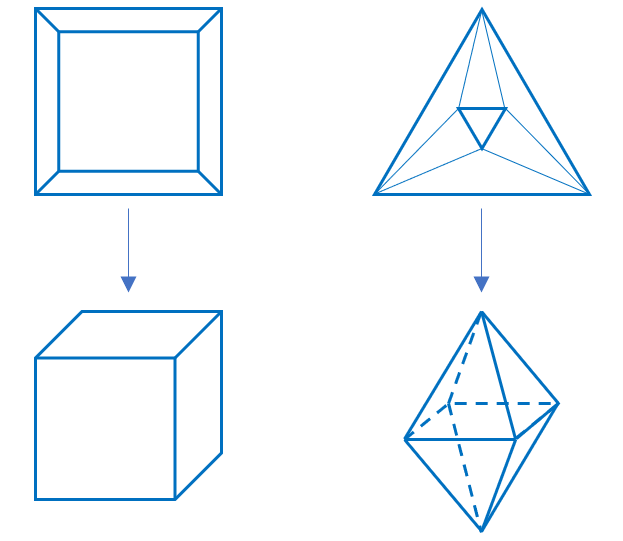
\includegraphics[width=0.35\textwidth]{figure/polytopal.png}}
      \caption{Examples of polytopals}
      \label{poly}
    \end{figure}
 \end{theorem}
    



  \begin{question}
    Minor means that  some subgraph of C contracts to A. Contraction is a surjective relationship. Subgraph means that you have to remove some components or remain the graph unchanged. 
    So \left |V_{A}  \right |\leq \left |V_{C}  \right | and \left |E_{A}  \right |\leq \left |E_{C}  \right |.
  \end{question}
  
  
  \begin{question}
    A is a minor of B and B is a minor of A.From question 1 we can get \[\left |V_{A}  \right |\leq \left |V_{B}  \right | \ \left |V_{B}  \right |\leq \left |V_{A}  \right |\] The only case is that \[\left |V_{A}  \right |= \left |V_{B}  \right |\]
    We can also get that edges are equal too.If we contract or remove any edges, we can't get the same number of vertices and edges. A is a subgraph of B, and B is a subgraph of A. A and B must be isormorphic.
  \end{question}
  
  \begin{question}
    Since all subdivisions or contractions are made of single subdivision or contraction, condition in figure \ref{prob3} is enough. The reverse action of a subdivision is actually a contraction. So the topological minor is also a special case of minor.
    \begin{figure}[!h]
      \centering
      {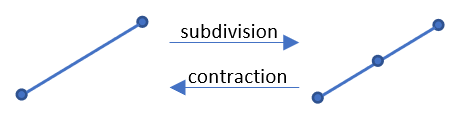
\includegraphics[width=0.4\textwidth]{figure/problem3.png}}
      \caption{Question 3}
      \label{prob3}
    \end{figure}
  \end{question}
  
  \begin{question}
  \begin{figure}[!h]
      \centering
      {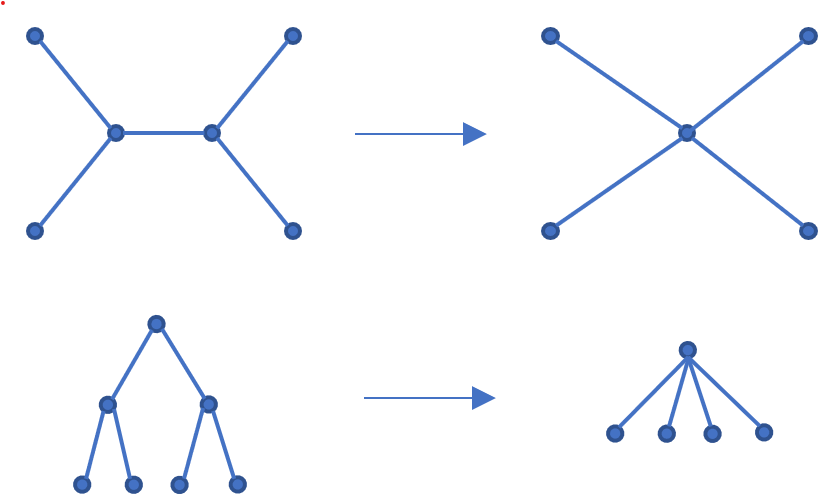
\includegraphics[width=0.30\textwidth]{figure/problem4.png}}
      \caption{Examples of question 4}
      \label{prob4}
    \end{figure}
  
  Give an example of a pair of trees \(A\) and \(B\) such that \(A \preceq B\), but
\(A\) is not a topological minor of \(B\). One way to think of it is to find a minor that can change the degree of vertices. The examples in figure \ref{prob4} both have a vertex with degree of 4 by contract vertices.
  \end{question}
    
  \begin{question}
    (Question 9 in homework3)
    If \(N(u)\cap N(v) = \varnothing \), there is no common neighbour of \(u\) and \(v\). In this way, the contraction of \((u,v)\) can only delete one vertex and one edge, then \(e(G) = e(H)\). The only way contraction could cause \(e(G) \neq e(H)\) is \(u\) and \(v\) have at least one neighbour, as shown in figure \ref{prob9}.
    \begin{figure}[!h]
      \centering
      {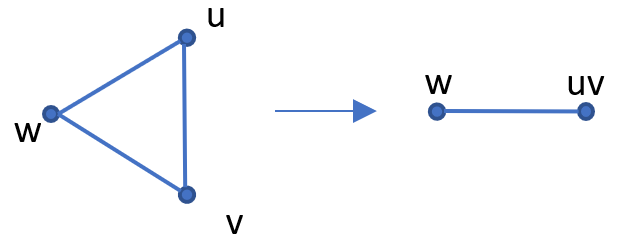
\includegraphics[width=0.5\textwidth]{figure/problem9.png}}
      \caption{Example of question 9}
      \label{prob9}
    \end{figure}

  \end{question}

\end{document}
